\subsection{(10\%) Bezier motion}
Scalars in bezier curves can befound by factoring Bernstein polynomials: BL = $((1-t) + t)^L$ for a bezier curve with L + 1 control points.

The camerais moved along a bezier curve with 4 control points.
\begin{itemize}
    \item[P1:] (7, 3, 2)
    \item[P2:] (18, 3, 5)
    \item[P3:] (15, 3, 8)
    \item[P4:] (9, 3, 11)
\end{itemize}

The motion should start 14 seconds after the program starts and it should end 24 seconds later, 38 seconds after the program starts.

\subsubsection{What is the camera's position 22 seconds after the program started?}

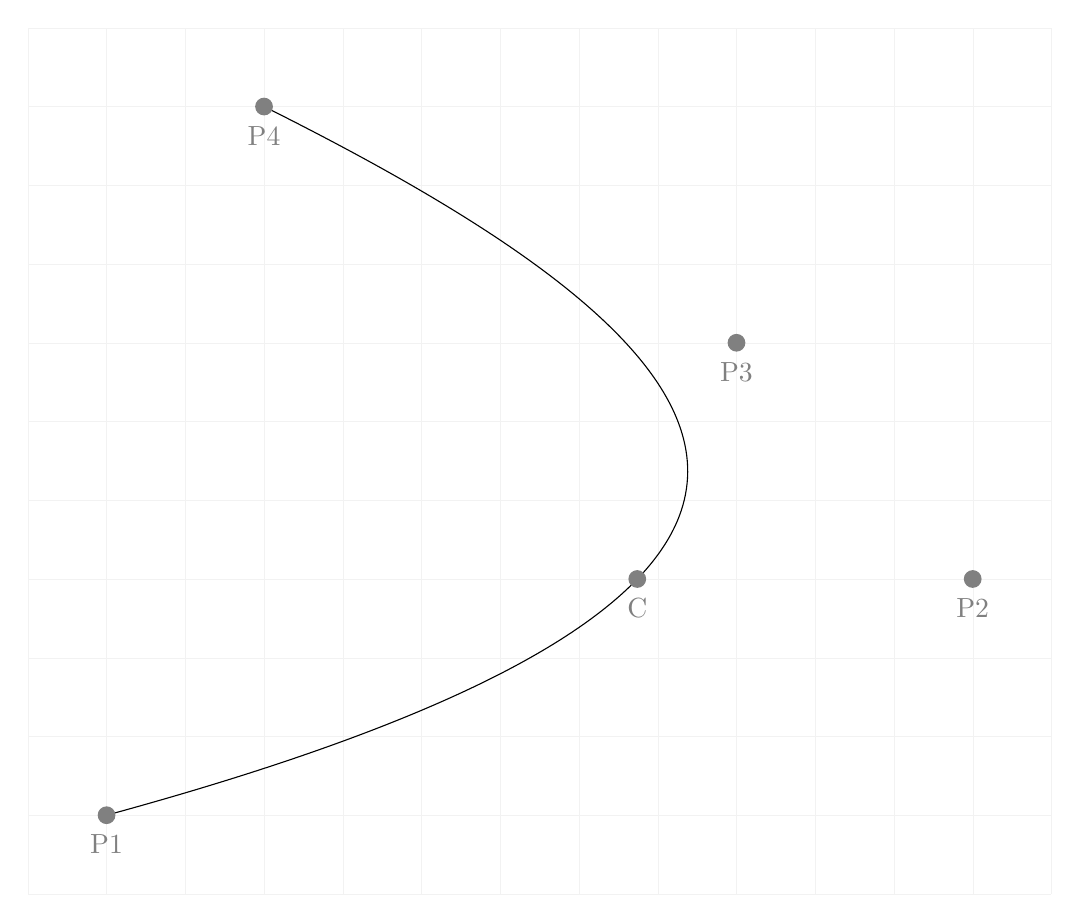
\begin{tikzpicture}[scale=1.0]
    \draw[step=1.0cm, gray!10, ultra thin](6, 1) grid (19, 12);
    \coordinate (P1) at ( 7,  2);
    \coordinate (P2) at (18,  5);
    \coordinate (P3) at (15,  8);
    \coordinate (P4) at ( 9, 11);
    \coordinate (C)  at (13.74, 5);


    \draw (P1) .. controls (P2) and (P3) .. (P4);
    
    \filldraw [gray] (P1) circle (3pt) node[label={below:P1}]{};
    \filldraw [gray] (P2) circle (3pt) node[label={below:P2}]{};
    \filldraw [gray] (P3) circle (3pt) node[label={below:P3}]{};
    \filldraw [gray] (P4) circle (3pt) node[label={below:P4}]{};
    \filldraw [gray] (C) circle (3pt) node[label={below:C}]{};

\end{tikzpicture}

$
    t
=
    \frac{t_{now} - t_{start}}{t_{duration}}
=
    \frac{22 - 14}{24}
=
    \frac{1}{3}
$

$
    P
=
        (1-t)^3 * t^0 * P1 +
    3 * (1-t)^2 * t^1 * P2 +
    3 * (1-t)^1 * t^2 * P3 +
        (1-t)^0 * t^3 * P4
$

$
    P
=
    \frac{8}{27} * \left(\begin{array}{c}7\\3\\2\end{array}\right)+
    \frac{4}{9} * \left(\begin{array}{c}18\\3\\5\end{array}\right)+
    \frac{2}{9} * \left(\begin{array}{c}15\\3\\8\end{array}\right)+
    \frac{1}{27} * \left(\begin{array}{c}9\\3\\11\end{array}\right)
$

$
    P
=
    \left(\begin{array}{c}
        13.74\\
        3\\
        5
    \end{array}\right)
$